\documentclass[12pt]{article}
\usepackage{graphicx}
\usepackage{amsmath}
\usepackage{braket}
\usepackage{mathtools}
\usepackage{subcaption}
\usepackage{multicol}
\usepackage{hyperref}
\usepackage{listings}
\usepackage{color}


\definecolor{mygrey}{rgb}{0.9,0.9,0.9}
\lstset{ backgroundcolor=\color{mygrey}} 


\usepackage[margin=1.0in]{geometry}


\begin{document}

\begin{center}{\Huge{\textbf{M.O.B}}} \end{center}

\begin{center} \textit{A 3-level Production}\end{center}


\begin{multicols}{2}

\textbf{Download.}

{\footnotesize{\url{https://github.com/3LP/M.O.B}}}

\vspace{0.25cm}

\textbf{What is M.O.B?}  M.O.B in it's original form is an IDE that combines both a computer terminal and a source code editor in one window.  We made M.O.B to give scientists with some programming skills, a basic GUI that they can use as a foundation to make their own apps.

\indent M.O.B is written in Python because it can be used to make many different applications, and it is one of the easier programming languages to pick up in order to do computing for science.  M.O.B uses Gtk3+ because there is great documentation for GUI design in Python, with this API.  Gtk3+ allows M.O.B to be cross-platform between Mac and Linux machines.  For Mac users, we highly recommend using homebrew and pypi to manage M.O.B core dependencies.   


\textbf{Dependencies.} Vte, Gtk3,  GLib, Gdk, GObject, Pango, PangoCairo, numpy, GtkSource, GnomeCommon, Gnome-doc-util, GnomeIconTheme, py2app.


\textbf{Development.} M.O.B could not have been built without the guidance provided by the Stack Exchange community. and this tutorial:  {\footnotesize{\url{http://www.dreamincode.net/forums/topic/150162-a-simple-text-editor-in-pythonpygtk/}}}


\indent The following link is a valuable resource when you are trying to incorporate your own app into M.O.B:    {\footnotesize{\url{https://python-gtk-3-tutorial.readthedocs.org/en/latest/}}}
 
 
\textbf{Why M.O.B?}  Making apps in Python is not difficult, however figuring out how to make a GUI for the first time will be .  First, you want to figure out what platform you want your app to run on. Next, you must research APIs that will satisfy your need's best.  Last, you have to write the code for your app.  There is a lot of unnecessary groundwork that you must do, M.O.B is here so you don't have to start from scratch.  M.O.B is provided with a tutorial so that developers can have an understanding of it's original structure.  The tutorials are there to get you up to speed on the layout of code for a GUI in Python, so that you can customize M.O.B to meet your computational desires.  

\end{multicols}

\vspace{0.05cm}

\begin{center}
\begin{minipage}[b]{0.66\linewidth}
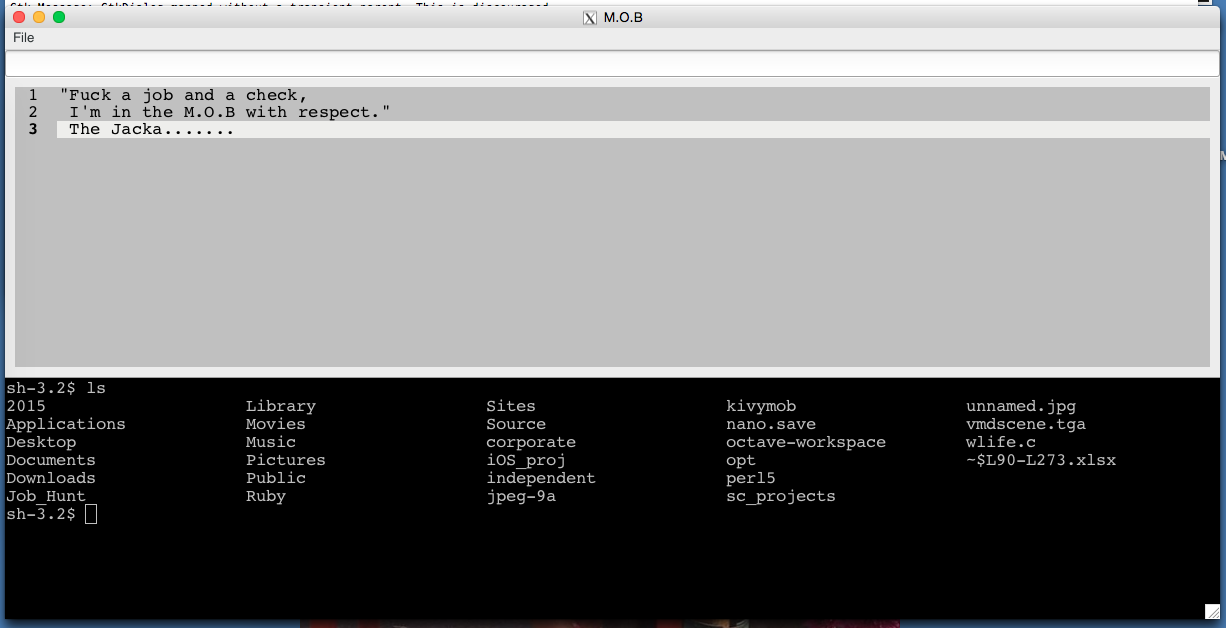
\includegraphics[width=\textwidth]{/Users/jacksonchiefelk/independent/M.O.B/screenshot.png}
\end{minipage}
\end{center}

\vspace{0.05cm}

\begin{center}{\footnotesize{\textbf{Figure 1.}  M.O.B screenshot.}} \end{center} 

\vspace{0.3cm}



\begin{center}{\Large{\textbf{IDE M.O.B Tutorial}}}\end{center}
{\footnotesize{
\begin{lstlisting}

import os,sys
from gi.repository import Gtk, Vte,Pango,PangoCairo
from gi.repository import GLib, Gdk
from gi.repository import GObject
from gi.repository import GtkSource

\end{lstlisting}
}}

\vspace{0.3cm}

\textbf{Figure 2.}  Minimal dependencies for the M.O.B IDE.  If you are interested in removing these from M.O.B to replace with your own app, you will not need GtkSource. 

\vspace{0.4cm}

\indent Before the class MainWindow is defined, we need to declare any classes that you will need to build your app.  For the IDE M.O.B, below are the classes that we need.

{\footnotesize{
\begin{lstlisting}

StatusBar = Gtk.Statusbar()
source = GtkSource.View()
buffer = source.get_buffer()
terminal = Vte.Terminal()
textview = Gtk.TextView()
entry = Gtk.Entry()
menu = Gtk.MenuBar()
filemenu = Gtk.Menu()
scrolledwindow1 = Gtk.ScrolledWindow()
vpaned = Gtk.VPaned()
grid = Gtk.Grid()


\end{lstlisting}    
}}


\vspace{0.3cm}


\textbf{Figure 3.} Declaring instances of required classes


\vspace{0.4cm}

\indent We have set the class MainWindow to inherit functions from Gtk.Window.  This class is the foundation of the GUI.  It contains the methods necessary to recreate classic GUI functionality; \textit{i.e.} it creates a window with a menubar, that can perform basic Open/Save/SaveAs/Exit functions.  


{\footnotesize{
\begin{lstlisting}

class MainWindow(Gtk.Window):
    file_tag = "''		
    # Name of File for Open/Save/SaveAs Functions
   
    def open_file(menuitem, user_param):
    	# Code specific to your application
    def save_file(menuitem,user_param):   
    	# Code specific to your application
    def save_file_as(menuitem,user_param):
    	# Code specific to your application
    def entry_go(self,widget):
	# Automatic code generator
	# Convert Latex to formulas into Python and/or C for loops
    def __init__(self):
        Gtk.Window.__init__(self)
        # Window title and Icon
        self.set_title("M.O.B")
        self.connect("delete-event", Gtk.main_quit)
        # IDE M.O.B specific code
     
#Starting Window
window = MainWindow()
Gtk.main()

\end{lstlisting}

}}

\vspace{0.3cm}


\textbf{Figure 4.} MainWindow Class.  


\vspace{0.3cm}

\indent Most of the code in figure 4 is missing, however this figure shows the basic structure for a M.O.B app.  See the source code on IDE M.O.B or your favorite IDE of choice.  The original M.O.B developer just wanted to write code in an app that combined a terminal and a source editor, in ONE window. 

\indent We are currently making an executable icon for Mac, so to use M.O.B you have to open it using the following terminal
command.

{\footnotesize{
\begin{lstlisting} 
python mob.py
\end{lstlisting}
}}

\end{document}